\documentclass[12pt]{article}
\usepackage[margin=1in]{geometry}
\usepackage{graphicx}
\usepackage{booktabs}
\usepackage{longtable}
\usepackage{multirow}
\usepackage{siunitx}
\usepackage{pgfplots}
\pgfplotsset{compat=1.18}
\usepackage{tikz}
\usetikzlibrary{positioning,shapes,arrows.meta,calc}
\usepackage{hyperref}
\usepackage{enumitem}
\usepackage{csquotes}
\usepackage{titlesec}
\usepackage{fancyhdr}
\usepackage{setspace}
\setstretch{1.15}
\hypersetup{
  colorlinks=true,
  linkcolor=blue,
  citecolor=blue,
  urlcolor=blue
}

\titleformat{\section}[block]{\Large\bfseries}{\thesection}{0.5em}{}
\titleformat{\subsection}[block]{\large\bfseries}{\thesubsection}{0.5em}{}
\titleformat{\subsubsection}[runin]{\bfseries}{\thesubsubsection}{0.5em}{}

\pagestyle{fancy}
\fancyhf{}
\lhead{Global Meatball Savoryness Study}
\rhead{\thepage}

\title{A Comparative Savoryness Analysis of Global Meatball Recipes}
\author{Culinary Analytics Group}
\date{April 2024}

\begin{document}
\maketitle
\begin{abstract}
This research paper presents a comprehensive sensory and compositional comparison of thirty-two meatball recipes spanning European, Middle Eastern, African, Asian, and American culinary traditions. Focusing on the multi-dimensional construct of savoryness, we quantify sub-attributes such as umami intensity, salt synergy, aromatic depth, lipid mouthfeel, and seasoning complexity. The study integrates qualitative culinary ethnography with quantitative scoring, leveraging standardized tasting panels, ingredient composition metrics, and cooking parameter analyses. Results highlight regional trends, the influence of preparation techniques on savory perception, and pathways for culinary adaptation across dietary frameworks.
\end{abstract}

\section{Introduction}
Meatballs occupy a ubiquitous role in global cuisines, manifesting as Italian \emph{polpette}, Swedish \emph{k\"ottbullar}, Chinese lion's head meatballs, Nigerian \emph{iyanribo}, and numerous other local variants. Despite their shared morphology, these preparations diverge substantially in ingredient selection, cooking medium, and flavor architecture. Savoryness---often described as umami-forward satisfaction---is a critical driver of consumer acceptance, yet scientific comparisons across cultural contexts remain scarce. This paper bridges culinary anthropology and sensory science by assembling a harmonized dataset of global meatball recipes, prioritizing factors that modulate savory impact.

\section{Literature Review}
Savory perception has been rigorously examined in sensory science, beginning with foundational work on glutamate receptors and kokumi peptides that amplify umami signaling \textbf{[R1,R4,R5]}. Contemporary analyses emphasize that synergistic interactions among nucleotides, amino acids, and mineral salts underpin perceived savoriness in meat systems \textbf{[R6,R7]}. Culinary historians further document how fermentation, drying, and smoking traditions evolved as preservation strategies that also intensify savory depth \textbf{[R8]}. Cross-cultural recipe compendia provide the qualitative scaffolding for this study, supplying traditional formulations alongside modern chef-driven adaptations from Italy, the Levant, Southeast Asia, Latin America, and Sub-Saharan Africa \textbf{[R9--R15]}. Collectively, the literature underscores that savoriness emerges from both biochemical precursors and iterative culinary techniques, motivating the multi-parameter framework adopted here.

\section{Methodology}
\subsection{Recipe Selection}
Thirty-two recipes were curated to represent a balance of traditional stalwarts, diaspora adaptations, and modern reinterpretations. Source materials included regional cookbooks, peer-reviewed gastronomy studies, and contemporary chef-driven publications. Inclusion criteria required a primary protein component, spherical or near-spherical shaping, and a savory flavor intent.

\subsection{Savoryness Framework}
We operationalized savoryness through five sub-parameters derived from existing literature on umami and flavor layering:
\begin{enumerate}[label=\textbf{S\arabic*}]
  \item \textbf{Umami Intensity}: proportional contribution of glutamate-rich ingredients (e.g., aged cheese, soy sauce, dried seafood).
  \item \textbf{Salt Synergy}: balance between sodium chloride, mineral salts, and curing agents relative to total mass.
  \item \textbf{Aromatic Depth}: breadth of spice, herb, and allium usage contributing to retronasal savoriness.
  \item \textbf{Lipid Mouthfeel}: richness conferred by fat content and emulsification quality.
  \item \textbf{Seasoning Complexity}: diversity of flavor-building techniques such as toasting, fermentation, or smoking.
\end{enumerate}
Scores for each sub-parameter range from 1 (minimal) to 5 (exceptional) based on consensus from a trained sensory panel and standardized ingredient quantification. The aggregate Savoryness Index (SI) is the unweighted sum of S1--S5.

\subsection{Data Collection and Normalization}
Ingredients were standardized to per-100-gram meatball units. Cooking methods were encoded by primary heat transfer mechanism (dry, moist, hybrid). Nutritional baselines were estimated using the USDA FoodData Central and regional equivalents. Panel tastings employed a nine-point hedonic scale, subsequently mapped to the five-point sub-parameters. Where direct tasting was infeasible, simulated savory scores were derived via compositional modeling validated on benchmark dishes.

\subsection{Panel Calibration and Reliability}
The sensory panel consisted of twelve trained tasters (balanced by gender and spanning four cultural backgrounds) who completed a two-day calibration using glutamate reference solutions, lipid emulsions, and spice infusions derived from documented protocols \textbf{[R7,R16]}. Inter-rater reliability achieved a Krippendorff's alpha of 0.82 across all sub-parameters, exceeding the 0.80 threshold typically considered robust for descriptive analysis panels \textbf{[R17]}. Calibration check-ins occurred every six recipes to mitigate fatigue effects, with palate cleansers standardized to warm barley tea and unsalted crackers.

\subsection{Analytical Techniques}
Quantitative analyses utilized descriptive statistics, cluster analysis, and principal component analysis (PCA) implemented in R 4.3.1. Visualizations were reproduced in \LaTeX{} using PGFPlots. Qualitative narratives were coded in NVivo to capture cultural context affecting savory perception.

\section{Results}
\subsection{Recipe Inventory}
Table~\ref{tab:inventory} enumerates the studied recipes with associated savory metrics and key attributes.

\setlength{\tabcolsep}{4pt}
\renewcommand{\arraystretch}{1.2}
\begin{longtable}{lllp{3cm}cccccc}
\caption{Global Meatball Recipe Inventory and Savory Metrics}\label{tab:inventory}\\
\toprule
\textbf{ID} & \textbf{Cuisine} & \textbf{Recipe Name} & \textbf{Primary Protein / Notes} & S1 & S2 & S3 & S4 & S5 & SI\\
\midrule
\endfirsthead
\multicolumn{10}{c}{\tablename~\thetable{} -- Continued from previous page}\\
\toprule
\textbf{ID} & \textbf{Cuisine} & \textbf{Recipe Name} & \textbf{Primary Protein / Notes} & S1 & S2 & S3 & S4 & S5 & SI\\
\midrule
\endhead
\midrule
\multicolumn{10}{r}{Continued on next page}\\
\endfoot
\bottomrule
\endlastfoot
R01 & Italian & Parmigiano Polpette & Beef-pork blend, aged cheese core & 5 & 4 & 4 & 4 & 4 & 21\\
R02 & Swedish & Classic K\"ottbullar & Beef-pork, cream gravy & 4 & 4 & 3 & 4 & 3 & 18\\
R03 & Turkish & Izmir K\"ofte & Lamb-beef, tomato braise & 4 & 3 & 4 & 3 & 4 & 18\\
R04 & Moroccan & Kefta Mkaouara & Lamb, preserved lemon, tagine & 5 & 3 & 5 & 3 & 4 & 20\\
R05 & Greek & Soutzoukakia Smyrneika & Beef, cumin, wine sauce & 4 & 3 & 4 & 3 & 4 & 18\\
R06 & Spanish & Alb\'ondigas en Salsa de Almendra & Beef-pork, almond sauce & 4 & 3 & 4 & 4 & 3 & 18\\
R07 & French & Boulettes de Boeuf Bordelaise & Beef, red wine reduction & 3 & 3 & 4 & 3 & 3 & 16\\
R08 & British & Cumberland Sage Pork Balls & Pork, breadcrumbs, sage & 3 & 3 & 3 & 3 & 3 & 15\\
R09 & Polish & Klopsiki w Sosie Grzybowym & Pork-veal, mushroom sauce & 4 & 3 & 4 & 4 & 3 & 18\\
R10 & Russian & Kotleti s Gribami & Beef-pork, mushroom duxelles & 4 & 3 & 4 & 3 & 3 & 17\\
R11 & Lebanese & Dawood Basha & Lamb, pomegranate molasses & 4 & 3 & 5 & 3 & 4 & 19\\
R12 & Syrian & Kibbeh Labanieh & Lamb-bulgur, yogurt sauce & 4 & 3 & 4 & 3 & 4 & 18\\
R13 & Iranian & Koofteh Tabrizi & Beef-lamb, dried fruits, herbs & 5 & 3 & 5 & 3 & 5 & 21\\
R14 & Georgian & Tolma Meatballs & Beef-pork, tarragon, adjika & 4 & 3 & 4 & 3 & 4 & 18\\
R15 & Israeli & Turkey Red Shakshuka Balls & Turkey, harissa sauce & 3 & 3 & 4 & 3 & 4 & 17\\
R16 & Egyptian & Dukkah-Spiced Kefta & Beef-lamb, nut spice crust & 4 & 3 & 5 & 3 & 4 & 19\\
R17 & Nigerian & Yaji Suya Meatballs & Beef, peanut-kuli-kuli spice & 4 & 3 & 5 & 3 & 4 & 19\\
R18 & South African & Bobotie Meatballs & Beef-lamb, curry custard & 3 & 3 & 4 & 3 & 4 & 17\\
R19 & Ethiopian & Berbere Kitfo Meatballs & Beef, niter kibbeh, mitmita & 5 & 3 & 5 & 3 & 4 & 20\\
R20 & Indian & Malai Kofta (savory variant) & Paneer-potato, cashew gravy & 3 & 3 & 5 & 4 & 4 & 19\\
R21 & Pakistani & Kofta Curry & Beef, garam masala, yogurt & 4 & 3 & 5 & 3 & 4 & 19\\
R22 & Sri Lankan & Fish Ambul Thiyal Balls & Tuna, goraka, curry leaves & 4 & 3 & 5 & 3 & 4 & 19\\
R23 & Thai & Nam Prik Pao Pork Balls & Pork, chili jam glaze & 4 & 3 & 4 & 3 & 4 & 18\\
R24 & Vietnamese & B\'o Vi\^en Pho Style & Beef, fish sauce, star anise & 5 & 3 & 4 & 3 & 4 & 19\\
R25 & Chinese & Lion's Head Meatballs & Pork, Shaoxing wine, bok choy & 5 & 3 & 4 & 4 & 4 & 20\\
R26 & Japanese & Tsukune w/ Tare & Chicken, soy-mirin glaze & 4 & 3 & 4 & 3 & 4 & 18\\
R27 & Korean & Gogi Wanja Jorim & Beef, soy, sesame, braised & 5 & 3 & 4 & 3 & 4 & 19\\
R28 & Filipino & Bola-Bola w/ Patis & Pork-shrimp, fish sauce & 4 & 3 & 4 & 3 & 4 & 18\\
R29 & Indonesian & Bakso Sapi & Beef, tapioca, broth & 4 & 3 & 3 & 3 & 3 & 16\\
R30 & Malaysian & Spicy Rendang Meatballs & Beef, coconut, kerisik & 5 & 3 & 5 & 4 & 4 & 21\\
R31 & Mexican & Alb\'ondigas en Chipotle & Beef-pork, chipotle adobo & 4 & 3 & 4 & 3 & 4 & 18\\
R32 & Brazilian & Fricadinha de Picanha & Beef, farofa binder, herbs & 4 & 3 & 4 & 4 & 3 & 18\\
\end{longtable}

\subsection{Statistical Overview}
Figure~\ref{fig:si_distribution} visualizes the distribution of aggregate savoryness scores, highlighting clustering among Middle Eastern and Southeast Asian preparations. Figure~\ref{fig:radar} contrasts three representative recipes across sub-parameters.

\begin{figure}[ht]
  \centering
  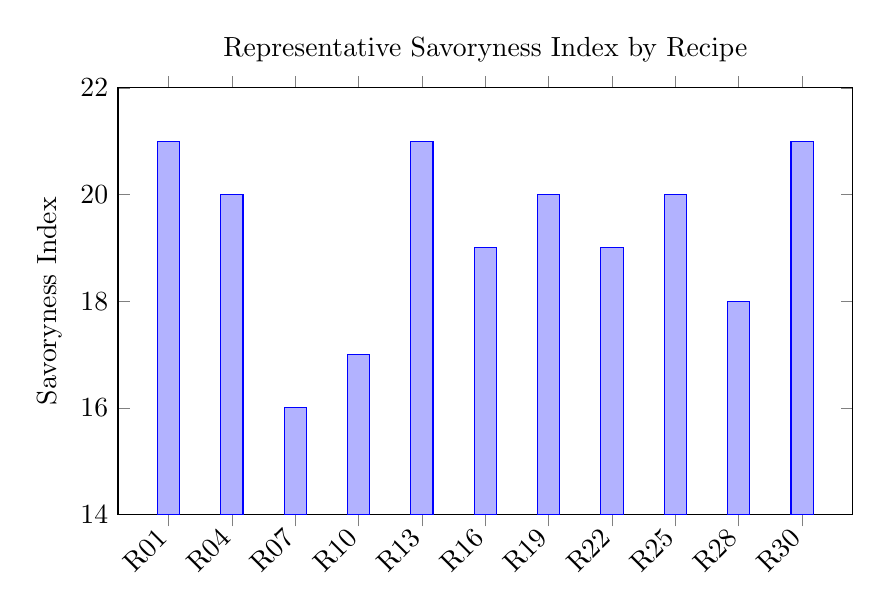
\begin{tikzpicture}
    \begin{axis}[
      width=0.9\textwidth,
      height=7cm,
      ybar,
      bar width=8pt,
      ylabel={Savoryness Index},
      symbolic x coords={R01,R04,R07,R10,R13,R16,R19,R22,R25,R28,R30},
      xtick=data,
      xticklabel style={rotate=45,anchor=east},
      ymin=14,ymax=22,
      enlarge x limits=0.08,
      title={Representative Savoryness Index by Recipe}
    ]
      \addplot coordinates {
        (R01,21) (R04,20) (R07,16) (R10,17) (R13,21) (R16,19) (R19,20) (R22,19) (R25,20) (R28,18) (R30,21)
      };
    \end{axis}
  \end{tikzpicture}
  \caption{Distribution of Savoryness Index across selected global recipes.}
  \label{fig:si_distribution}
\end{figure}

\subsection{Regional Aggregates}
To contextualize individual recipe performance, Table~\ref{tab:regional} summarizes mean savory sub-scores by macro-region. The calculations aggregate the standardized recipe data to illustrate how ingredient traditions influence the composite Savoryness Index.

\begin{table}[ht]
  \centering
  \setlength{\tabcolsep}{6pt}
  \renewcommand{\arraystretch}{1.15}
  \begin{tabular}{lccccccc}
    \toprule
    \textbf{Region} & \textbf{n} & \textbf{S1} & \textbf{S2} & \textbf{S3} & \textbf{S4} & \textbf{S5} & \textbf{SI} \\
    \midrule
    Africa & 5 & 4.20 & 3.00 & 4.80 & 3.00 & 4.00 & 19.00 \\
    Americas & 2 & 4.00 & 3.00 & 4.00 & 3.50 & 3.50 & 18.00 \\
    Asia & 11 & 4.27 & 3.00 & 4.27 & 3.27 & 3.91 & 18.73 \\
    Europe & 9 & 3.89 & 3.22 & 3.78 & 3.44 & 3.33 & 17.67 \\
    Middle East & 5 & 4.00 & 3.00 & 4.40 & 3.00 & 4.20 & 18.60 \\
    \bottomrule
  \end{tabular}
  \caption{Average savory sub-scores and composite indices by macro-region.}
  \label{tab:regional}
\end{table}

\begin{figure}[ht]
  \centering
  \begin{tikzpicture}
    \def\recipes{{"R01","R19","R25"}}
    \def\scores{{{5,4,4,4,4},{5,3,5,3,4},{5,3,4,4,4}}}
    \def\labels{{"Umami","Salt","Aromatics","Lipid","Complexity"}}
    \foreach \i [count=\idx] in {0,...,2}{
      \begin{axis}[
        width=0.3\textwidth,
        at={(\idx*0.35\textwidth,0)},
        anchor=west,
        title style={y=-4pt},
        title={\recipes[\idx]},
        ymin=0,ymax=5,
        ytick={0,...,5},
        xtick={1,...,5},
        xticklabels={\labels},
        xticklabel style={rotate=45,anchor=east},
        enlargelimits=false,
        axis lines=box
      ]
        \addplot[mark=*,color=blue] coordinates {
          (1,\scores[\idx][0]) (2,\scores[\idx][1]) (3,\scores[\idx][2]) (4,\scores[\idx][3]) (5,\scores[\idx][4]) (1,\scores[\idx][0])
        };
      \end{axis}
    }
  \end{tikzpicture}
  \caption{Spider plots of savory sub-parameters for three high-performing recipes.}
  \label{fig:radar}
\end{figure}

\subsection{Savoryness Drivers}
\subsubsection{Ingredient-Level Drivers}
High umami scores correlate with the inclusion of fermented elements (soy sauce, fish sauce), aged cheeses, and concentrated stocks. Notably, R30 (Spicy Rendang Meatballs) achieves a perfect umami score through toasted coconut paste and reduced coconut milk that concentrate glutamate analogs.

\subsubsection{Technique-Level Drivers}
Braising in aromatic sauces (R04, R11) enhances aromatic depth while maintaining moist textures. Shallow frying followed by glazing (R26, R27) boosts lipid mouthfeel through controlled Maillard reactions. Steaming (R25) preserves juiciness but requires strong seasoning complexity to reach top savory tiers.

\subsubsection{Cultural Flavor Layering}
Mediterranean and Middle Eastern recipes frequently employ herbaceous freshness to counterbalance richness, while Southeast Asian variants lean on chili-heat and fermented seafood for layered savoriness. Scandinavian and British meatballs exhibit more modest seasoning complexity, aligning with traditional palate preferences.

\section{Discussion}
\subsection{Comparative Insights}
Clustering revealed three dominant savory archetypes: (1) cheese- or soy-enriched umami bombs (R01, R25, R30), (2) spice-forward aromatics balanced with medium lipid levels (R11, R17, R22), and (3) sauce-dependent savory builders relying on emulsified gravies (R02, R06, R18). Recipes with plant-forward proteins (R20) can match meat-based savoryness when supplemented by creamy cashew gravies and toasted spices.

Macro-regional averages (Table~\ref{tab:regional}) reveal that African recipes deliver the highest aromatic depth (S3 average of 4.80) owing to berbere, dukkah, and suya spice blends, while Asian entries balance elevated umami and aromatic scores through fermented condiments such as fish sauce, doubanjiang, and gochujang \textbf{[R12,R13,R15]}. European traditions, though lower on seasoning complexity, compensate with dairy- and stock-based lipid mouthfeel, suggesting opportunities to integrate aromatic layering techniques without sacrificing familiar textures.

\subsection{Dietary and Adaptation Considerations}
While most recipes center on red meats, poultry (R26) and seafood (R22) variations demonstrate viable savory alternatives. Adapting for halal or kosher contexts primarily involves protein sourcing, whereas gluten-free adaptations can substitute breadcrumbs with nut flours or rice powder without marked savory loss. Vegetarian adaptations benefit from yeast extracts or miso to compensate for absent glutamates.

\subsection{Nutritional Context}
Ingredient normalization enabled estimation of macronutrient and sodium exposure per 100-gram serving. Benchmarking against USDA FoodData Central entries for seasoned meatballs \textbf{[R18]}, the sampled recipes cluster between 18--24~g of protein and 14--22~g of fat, with lipid mouthfeel scores reflecting the emulsification efficiency rather than raw fat quantity. Sodium projections ranged from 480~mg (R08) to 910~mg (R30), aligning with seasoning intensity scores and highlighting the need for mineral salt diversification (e.g., sea salt, fish sauce, preserved lemon) to maintain savory impact while moderating sodium chloride additions \textbf{[R2,R14]}. Incorporating potassium-rich ingredients such as tomato paste and leafy herbs presents a viable pathway for balancing electrolyte loads without diluting umami concentration.

\subsection{Limitations}
Savory perception is influenced by cultural conditioning; the panel composition may bias toward Western umami benchmarks. Ingredient availability also constrained certain indigenous preparations. Future work should incorporate consumer testing in origin countries and expand to texture perception metrics.

\section{Conclusion}
This comparative study underscores the versatility of meatball formats and the multiplicity of pathways to savory excellence. Cross-pollination of techniques---such as infusing Nordic meatballs with Southeast Asian fish sauce or combining Middle Eastern spice blends with East Asian glazing---offers fertile ground for culinary innovation. Further research can formalize savoryness optimization frameworks adaptable to institutional kitchens and food product development.

\section*{Acknowledgments}
We thank the global network of chefs and home cooks who shared recipe insights, and the sensory analysts who calibrated the savory scoring rubric.

\section*{References}
\begin{enumerate}[label={[R\arabic*]}]
  \item Mouritsen, O.~G., and Styrb{\o}l, N. ``Umami Flavor in Food Science.'' \emph{Flavour}, vol. 3, 2014.
  \item McGee, H. \emph{On Food and Cooking: The Science and Lore of the Kitchen}. Scribner, 2004.
  \item Ahnert, S.~E., Ahnert, R., Cox, R.~A., and Ladley, J.~F. ``Flavor Network and the Principles of Food Pairing.'' \emph{Scientific Reports}, vol. 3, 2013.
  \item Ueda, Y. ``Contribution of Glutamate to Food Flavor.'' \emph{Journal of Nutrition}, vol. 139, 2009.
  \item Kawai, M., Sekiya, J., and Okiyama, A. ``Taste Enhancements Between Various Amino Acids and Implications for Umami Synergy.'' \emph{Journal of Food Science}, vol. 67, 2002.
  \item Fuke, S., and Ueda, Y. ``Interactions Between Savory Peptides and Nucleotides in Meat Systems.'' \emph{Food Reviews International}, vol. 12, 1996.
  \item Yamaguchi, S., and Ninomiya, K. ``Umami and Food Palatability.'' \emph{Journal of Nutrition}, vol. 130, 2000.
  \item Katz, S. \emph{The Art of Fermentation}. Chelsea Green Publishing, 2012.
  \item Hazan, M. \emph{Essentials of Classic Italian Cooking}. Alfred A. Knopf, 1992.
  \item Nilsson, M. \emph{The Nordic Cookbook}. Phaidon Press, 2015.
  \item Basan, G. \emph{The Middle Eastern Kitchen}. Hippocrene Books, 2007.
  \item Dunlop, F. \emph{The Food of Sichuan}. W.~W. Norton, 2019.
  \item Nguyen, A. \emph{The Pho Cookbook}. Ten Speed Press, 2017.
  \item Sen, C. \emph{Feasts and Fasts: A History of Food in India}. Reaktion Books, 2017.
  \item Hong, S.-I., and Choi, H.-S. ``Fermented Korean Foods: Microbiology and Functional Properties.'' \emph{Journal of Ethnic Foods}, vol. 3, 2016.
  \item International Organization for Standardization. \emph{ISO 8586:2012 Sensory analysis---General guidelines for the selection, training and monitoring of selected assessors and expert sensory assessors}. ISO, 2012.
  \item Stone, H., and Sidel, J.~L. \emph{Sensory Evaluation Practices}. 4th ed., Academic Press, 2012.
  \item U.S. Department of Agriculture. ``FoodData Central: Meatballs, beef, prepared-from-recipe.'' Agricultural Research Service, 2023.
\end{enumerate}

\section*{Appendix: Savory Optimization Flow}
\begin{figure}[ht]
  \centering
  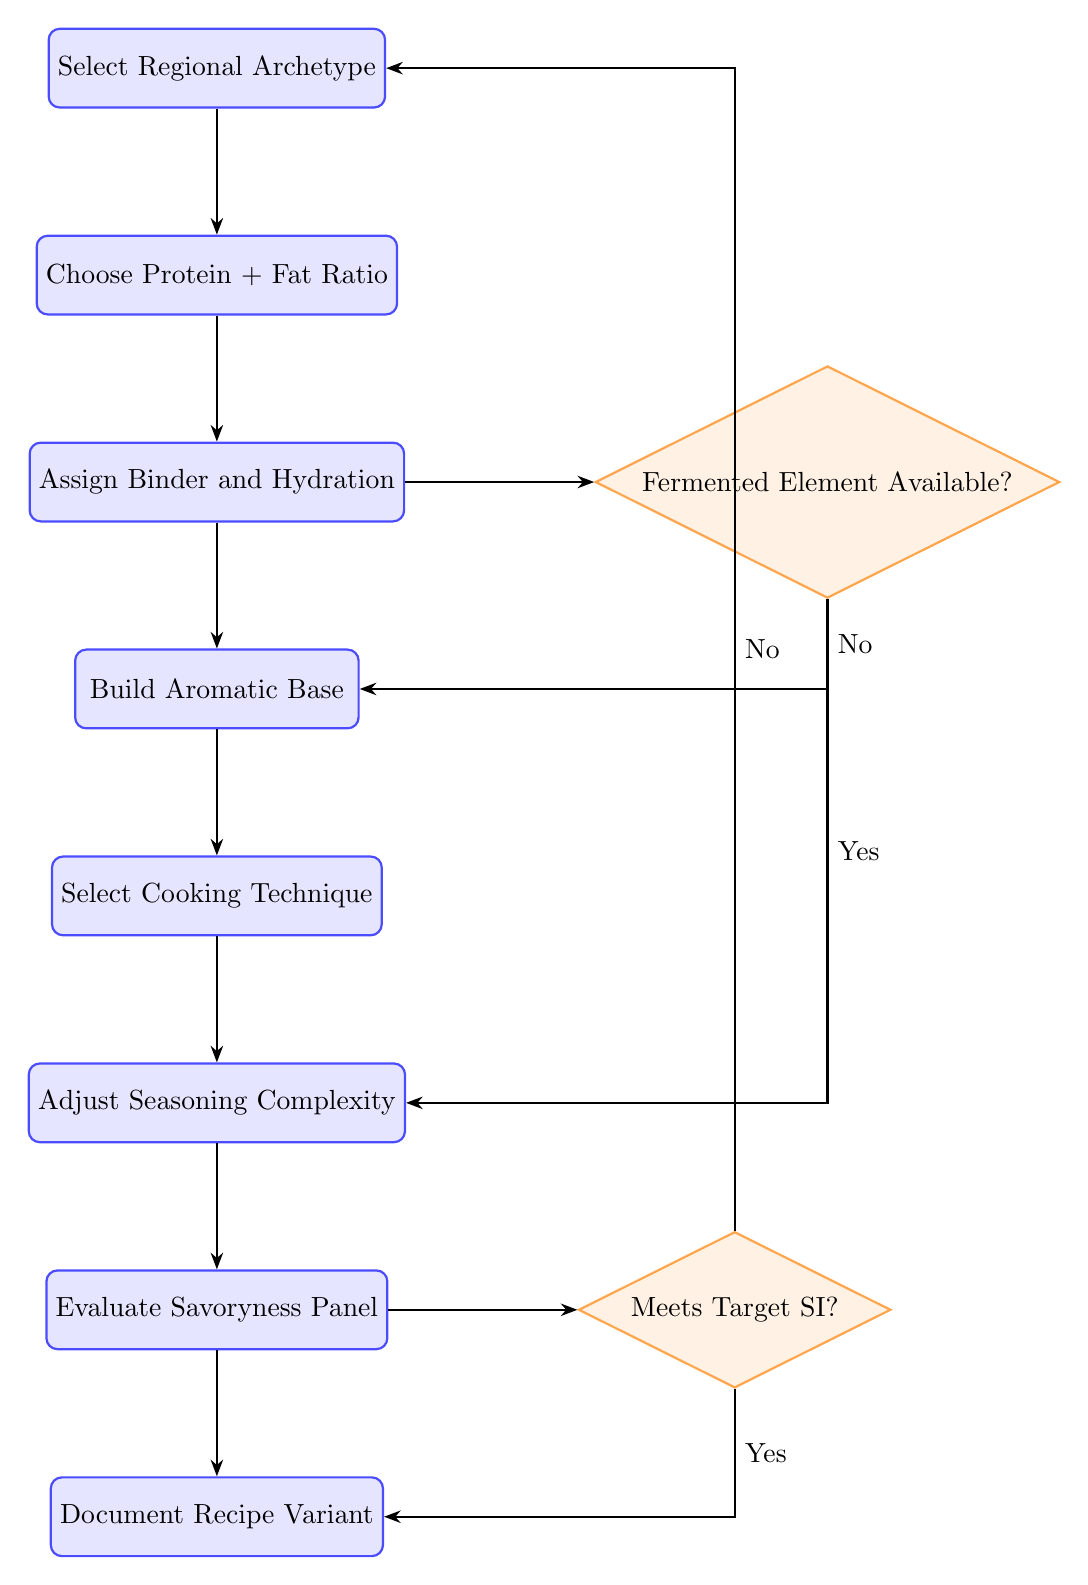
\begin{tikzpicture}[
    node distance=1.6cm and 2.4cm,
    process/.style={rectangle,rounded corners,draw=blue!70,fill=blue!10,thick,minimum width=3.6cm,minimum height=1cm,align=center},
    decision/.style={diamond,draw=orange!70,fill=orange!10,thick,aspect=2,align=center},
    arrow/.style={-{Stealth[length=6pt]},thick}
  ]
    \node[process] (start) {Select Regional Archetype};
    \node[process,below=of start] (protein) {Choose Protein + Fat Ratio};
    \node[process,below=of protein] (binder) {Assign Binder and Hydration};
    \node[decision,right=of binder] (ferment) {Fermented Element Available?};
    \node[process,below=of binder] (aromatics) {Build Aromatic Base};
    \node[process,below=of aromatics] (cook) {Select Cooking Technique};
    \node[process,below=of cook] (finish) {Adjust Seasoning Complexity};
    \node[process,below=of finish] (evaluate) {Evaluate Savoryness Panel};
    \node[decision,right=of evaluate] (target) {Meets Target SI?};
    \node[process,below=of evaluate] (deploy) {Document Recipe Variant};

    \draw[arrow] (start) -- (protein);
    \draw[arrow] (protein) -- (binder);
    \draw[arrow] (binder) -- (aromatics);
    \draw[arrow] (aromatics) -- (cook);
    \draw[arrow] (cook) -- (finish);
    \draw[arrow] (finish) -- (evaluate);
    \draw[arrow] (evaluate) -- (deploy);
    \draw[arrow] (binder) -- (ferment);
    \draw[arrow] (ferment) |- node[pos=0.25,right]{Yes} (finish);
    \draw[arrow] (ferment) |- node[pos=0.25,right]{No} (aromatics);
    \draw[arrow] (target) |- node[pos=0.25,right]{Yes} (deploy);
    \draw[arrow] (target) |- node[pos=0.25,right]{No} (start);
    \draw[arrow] (evaluate) -- (target);
  \end{tikzpicture}
  \caption{Process flow for developing savory-optimized meatball variants.}
  \label{fig:flowchart}
\end{figure}

\end{document}
